\chapter*{Dodatak} \label{chap:appendix}

\section*{Fundamentalni Principi 1889}

Kao što je drugdje već bilo navedeno, Adventisti Sedmog Dana nemaju kredo osim Biblije; ali se drže određenih dobro definiranih točaka vjere, za koje se osjećaju spremnima dati razlog “svakomu koji traži obrazloženje”. Sljedeće teze se mogu uzeti kao sažetak glavnih obilježja njihove vjere, nad kojima, koliko znamo, stoji jednoglasnost cijeloga tijela. Oni vjeruju, —

\lettrine{I.} Da postoji jedan Bog, osobno, duhovno biće, stvoritelj svih stvari, svemoguć, sveznajuć, i vječan; beskonačan u mudrosti, svetosti, pravednosti, dobroti, istini i milosti; nepromjenjiv, i svugdje prisutan po svojem predstavniku, Svetome Duhu. Psalam 139:7.

\lettrine{II.} Da postoji jedan Gospodin Isus Krist, Sin Vječnog Oca, Onaj po kojemu je On stvorio sve stvari, i po kojemu one postoje; da je On uzeo na sebe prirodu potomstva Abrahamova za otkupljenje naše pale rase; da je On prebivao među ljudima pun milosti i istine, živio nama za primjer, umro kao naša žrtva, uskrsnuo radi našeg opravdanja, bio uznesen u visine da bude naš posrednik u svetištu na Nebu, gdje kroz zasluge Svoje prolivene krvi osigurava pomirenje i oproštaj grijeha svima onima koji mu pokajnički dolaze; i da kao završni dio svoga djela kao svećenika, prije nego što preuzme svoje prijestolje kao kralj, učiniti će veliko pomirenje za grijehe svih takvih, i njihovi grijesi će tada biti izbrisani (Djela 3:19) i uklonjeni iz svetišta, kao što je pokazano u službi Levitskog svećenstva, koja je nagovještavala i oslikavala službu našega Gospodina na Nebu. Vidi Lev. 16; Heb 8:4,5; 9:6,7; itd.

\lettrine{III.} Da je Sveto Pismo Staroga i Novoga Zavjeta dâto nadahnućem Božjim, sadrži potpuno otkrivenje Njegove volje čovjeku, i ono je jedino nepogrešivo pravilo vjere i prakse.

\lettrine{IV.} Da je krštenje obred Kršćanske crkve, koje slijedi nakon vjere i pokajanja, — obred po kojemu proslavljamo uspomenu na Kristovo uskrsnuće, pa ovim činom prikazujemo svoju vjeru u Njegovu smrt i uskrsnuće, i kroz to, uskrsnuće svih svetih u posljednji dan; i da nijedan drugi način ne predstavlja prikladno ove činjenice osim onoga koje Pismo propisuje, naime, uronjavanjem. Rimljanima 6:3-5; Kološanima 2:12.

\lettrine{V.} Da novorođenje sadrži potpunu promjenu potrebnu da budemo učinjeni prikladnim za kraljevstvo Božje, i sastoji se od dva dijela: prvi, moralna promjena, izvršena obraćenjem i kršćanskim životom (Ivan 3:3,5); drugo, fizička promjena prilikom drugog Kristovog dolaska, čime, ako smo mrtvi, ustat ćemo neraspadljivi, i ako smo živi, promijenjeni u besmrtnost u trenutku, u treptaju oka. Luka 20:36, 1 Korinćanima 15:51, 52.

\lettrine{VI.} Da je proroštvo dio Božjeg otkrivenja čovjeku; da je uključeno u ono Pismo koje je korisno za poučavanje, (2 Timoteju 3:16); da je osmišljeno za nas i za našu djecu (Ponovljeni zakon 29:29); da je ono daleko od toga da je obavijeno u neprobojnu misteriju, i da je to ono što posebno sačinjava riječ Božju koja je svjetiljka našoj nozi i svjetlo našoj stazi, (Psalam 119:105; 2 Petrova 1:19); da je blagoslov izgovoren nad onima koji to proučavaju, (Otkrivenje 1:1-3); i zbog toga ono se mora razumjeti od strane naroda Božjega dovoljno da mu pokazuje njegov položaj u povijesti svijeta, i posebne dužnosti koje se zahtijevaju od njih.

\lettrine{VII.} Da povijest svijeta od naznačenih datuma u prošlosti, od dizanja i padanja carstava i kronološkog slijeda događaja pa do uspostavljanja Božjeg vječnog kraljevstva, su naznačeni u brojnim proročkim lancima; i da ta proročanstva su sada sva ispunjena osim završnih scena.

\lettrine{VIII.} Da je doktrina obraćenja svijeta i privremeni milenij bajka ovih posljednjih dana, predviđena da uspava ljude u stanje tjelesne sigurnosti i učini ih nespremnim za veliki dan Gospodnji koji dolazi kao lopov u noć (1 Sol. 5:3); da će drugi Kristov dolazak prethoditi, a ne uslijediti nakon milenija; jer dok se Gospodin ne pojavi, papska će sila, sa svim svojim grozotama, nastaviti (2 Sol. 2:8), pšenica i kukolj će rasti zajedno (Mat. 13:29,30,39), i zli ljudi i varalice napredovat će iz zla u gore, kao što riječ Božja objavljuje. 2. Tim 3:1,13.

\lettrine{IX.} Da se pogreška Adventista u 1844. tiče prirode događaja koji se tada dogodio, a ne vremena dešavanja; da ni jedan proročki period nije dat koji će dokučiti drugi dolazak, već da je najdulji od dvije tisuće tristo dana iz Dan. 8:14, završen 1844, i doveo nas do događaja zvanog čišćenje svetišta.

\lettrine{X.} Da je svetište novog saveza šator Božji na Nebu, o kojem Pavao govori u Hebrejima 8, pa nadalje, od kojeg je naš Gospodin, kao veliki svećenik, službenik; da je to svetište antitip Mojsijevog šatora, i da je svećenička služba našeg Gospodina povezana s njime, u tome što je ono antitip službe Židovskih svećenika od prijašnje raspodjele. (Heb. 8:1-5, itd.); da će to Svetište, a ne Zemlja, biti očišćeno na kraju dvije tisuće i tristo dana, što je naznačeno kao čišćenje u ovom slučaju, kao i u tipu, jednostavnim ulaskom velikog svećenika u Svetinju nad Svetinjama, da završi službu povezanu s tim, čineći pomirenje i uklanjajući iz svetišta grijehe koji su mu bili preneseni putem službe u prvom odjeljenju, (Lev 16, Heb. 9:22, 23); i da taj rad, u antitipu, koji započinje 1844., sačinjava pravo čišćenje grijeha vjernika (Djela 3:19), zauzima kratak, ali neodređen period, na čijem kraju je završen rad milosrđa za svijet i tada će uslijediti drugi Kristov dolazak.

\lettrine{XI.} Da su Božji moralni zahtjevi isti prema svim ljudima u svim vremenima; da su oni sažeto sadržani u zapovijedima koje je Jahve izgovorio sa Sinaja, uklesani na kamene ploče i pohranjeni u kovčeg, koji je posljedično nazvan “kovčeg saveza”, ili zavjet. (Brojevi. 10:33, Heb. 9:4), itd.; da je ovaj zakon nepromjenjiv i vječan, kao prijepis ploča pohranjenih u kovčegu u istinskom svetištu na visini, koji je iz istog razloga i nazvan kovčeg Božjeg zavjeta; rečeno nam je da je zvukom sedme trube “otvoren hram Božji na Nebu, i tamo se vidio kovčeg njegovog zavjeta”. Otkrivenje 11:19.

\lettrine{XII.} Da četvrta zapovijed ovog zakona zahtijeva da posvetimo sedmi dan svakog tjedna, koji se uobičajeno naziva subotom, suzdržavanjem od vlastitog rada, i obavljanjem svetih i vjerskih dužnosti; da je ovo jedina tjedna subota poznata Bibliji, kao dan koji je bio odvojen prije nego što je raj izgubljen, (Post. 2: 2, 3), i koji će se slaviti u obnovljenom raju, (Iza. 66:22, 23); da činjenice na kojima je institucija subote utemeljena su vezane za sedmi dan, dok one nisu istinite ni za jedan drugi dan; i da su pojmovi, židovski Šabat, kao što je primjenjeno na sedmi dan i kršćanski Šabat,kao što je primjenjeno na prvi dan tjedna, nazivi ljudskog izuma, zapravo ne biblijski i lažni u značenju.

\lettrine{XIII.} Da je čovjek grijeha, papstvo, promijenio vremena i zakone (Božji zakon, Dan 7:25), i zaveo gotovo cijelo kršćanstvo u pogledu četvrte zapovijedi, mi nalazimo proročanstvo o reformi u tom pogledu koja će biti dovedena među vjernike neposredno prije dolaska Krista. Iza. 56:1,2, 1 Pet. 1:5, Otk 14:12, itd.

\lettrine{XIV.} Da Kristovi sljedbenici trebaju biti osobit narod, koji ne slijede običaje, niti se prilagođavaju putovima svijeta; ne vole njegove užitke niti toleriraju njegove gluposti; jer apostol kaže da “tko god dakle poželi biti prijatelj svijetu” u tom smislu, “neprijateljem Božjim postaje” (Jak 4,4); i Krist kaže da ne možemo imati dva gospodara, ili istodobno služiti Bogu i mamonu. Mat. 6: 24.

\lettrine{XV.} Da Pisma inzistiraju na jednostavnosti i skromnosti odjeće kao istaknutog znaka učeništva u onima koji tvrde da su sljedbenici Onoga koji je bio “krotak i ponizan u srcu”; da nošenje zlata, biserja i skupih odijela, ili bilo što što je dizajnirano samo da ukrašava osobu i potiče ponos tjelesnog srca, treba odbaciti, prema spisima kao što su 1 Tim.2: 9,10; 1. Petrova 3:3,4.

\lettrine{XVI.} Da sredstva za potporu evanđeoskoga rada među ljudima bi trebala biti priložena iz ljubavi prema Bogu i ljubavi prema dušama, a ne sakupljena iz crkvenih lutrija, ili iz prigoda osmišljenih da pridonose zabavnim i apetitom vođenim sklonostima grešnika, poput sajmova, festivala, kamenica za večeru, čaja, metli, magaraca, i ludih druženja itd., što je sramota Kristovoj crkvi; da udio nečijeg dohotka u prijašnjim dispenzacijama ne može biti ništa manji pod evanđeljem; da je isti koliko i Abrahamov (čija smo djeca, ako smo Kristovi, Gal 3,29) kada je dao Melkisedeku (tip Krista) kada mu je dao desetinu od svega (Heb 7: 1-4); desetina je Gospodinova (Lev 27:30); i taj deseti dio prihoda također treba nadopuniti darovima od onih koji su sposobni poduprijeti evanđelje. 2 kor. 9: 6; Mal. 3: 8, 10.

\lettrine{XVII.} Da je tjelesno srce u neprijateljstvu prema Bogu i njegovu zakonu, to neprijateljstvo može biti podčinjeno samo korjenitom promjenom sklonosti, zamjenom nečasnih za sveta načela; da ova preobrazba praćena pokajanjem i vjerom, je poseban posao Duha Svetoga i sačinjava obnovu ili obraćenje.

\lettrine{XVIII.} Da su svi prekršili Božji zakon i ne mogu sami sebe učiniti poslušnima Njegovim pravednim zahtjevima, mi smo ovisni o Kristu, prvo, za opravdanje od naših prošlih prijestupa, i drugo, za milost pomoću koje ćemo izraziti prihvatljivu poslušnost njegovom svetom zakonu u vremenu koji dolazi.

\lettrine{XIX.} Da Duh je Božji obećan očitovati se u crkvi kroz određene darove, nabrojane posebno u 1. Kor. 12 i Ef. 4; da ti darovi nisu osmišljeni da istisnu ili zauzmu mjesto Biblije, koja je dovoljna da nas učini mudrim za spasenje, tako ni Biblija ne može preuzeti mjesto Duha Svetoga; da je u određivanju različitih kanala njegovog djelovanja, taj Duh jednostavno odredio vlastito postojanje i prisutnost s Božjim narodom do kraja vremena, da dovede do razumijevanja te riječi koje je nadahnuo, da uvjeri o grijehu, i čini preobrazbu u srcu i životu; i da oni koji uskraćuju Duhu svoje mjesto i djelovanje, jasno negiraju onaj dio Biblije koji joj dodjeljuje taj posao i položaj.

\lettrine{XX.} Da Bog, u skladu s njegovim ujednačenim postupanjem sa rasom, šalje proglas približavanja drugog Kristovog dolaska; i da je taj rad simboliziran trima vijestima iz Otkrivenja 14, od kojih posljednja donosi pogled na djelo reforme Božjeg zakona, da njegov narod može steći potpunu spremnost za taj događaj.

\lettrine{XXI.} Da vrijeme čišćenja svetišta (pogledaj propoziciju X.), koje je sinkronizirano sa vremenom objavljivanja treće vijesti (Otk. 14:9, 10), je vrijeme istražnog suda, prvo u odnosu na mrtve, i drugo, na kraju vremena milosti, u odnosu na žive, kako bi odredili tko od mnoštva koji sada spavaju u prahu zemaljskom su dostojni imati udio u prvom uskrsnuću, i tko od živog mnoštva je dostojan uzašašća,— točke koje se moraju utvrditi prije pojave Gospodina.

\lettrine{XXII.} Da grob, kuda svi naginjemo, izražen hebrejskom riječi šeol i grčkom riječi had, je mjesto ili stanje u kojem nema rada, umovanja, mudrosti ni znanja. Propovjednik 9:10.

\lettrine{XXIII.} Da stanje na koje smo svedeni smrću je stanje tišine, neaktivnosti i potpune besvijesti. Psalam 146:4; Propovjednik 9:5, 6; Daniel 12:2.

\lettrine{XXIV.} Da će iz ove tamnice groba čovječanstvo biti dovedeno tjelesnim uskrsnućem; pravednici imajući udio u prvom uskrsnuću, koje se odvija tijekom drugog Kristovog dolaska; a zli u drugom uskrsnuću, koje će biti tisuću godina poslije. Otk. 20:4-6.

\lettrine{XXV.} Da će se na posljednju trubu živi pravednici promijeniti u trenutku, u treptaj oka, i s uskrslim pravednicima biti uzeti u susret Gospodinu u zrak, tako da zauvijek budu s Gospodinom. 1 Sol. 4:16, 17; 1 Kor. 15:51, 52.

\lettrine{XXVI.} Da su te besmrtne osobe tada uzete u Nebo, u Novi Jeruzalem, Očevu kuću u kojoj ima mnogo stanova (Ivan 14:1-3), gdje vladaju s Kristom tisuću godina, sudeći svijet i pale anđele, to jest, odmjeravaju kaznu koja će se izvršiti na njima na kraju tisuću godina (Otkrivenje 20:4; 1 Kor. 6:2, 3); da se u to vrijeme zemlja nalazi u opustošenom i kaotičnom stanju (Jer. 4:23-27), opisano, kao u početku, grčkom riječi abussos— “bezdan” (Septuaginta Post. 1:2); i da je ondje sotona vezan tijekom tisuću godina (Otkrivenje 20:1, 2), i ondje u konačnici uništen (Otk 20:10; Mal. 4:1); prikaz ruševine koju je napravio u svemiru, prikladno je učinjen, za neko vrijeme, njegovom turobnom tamnicom, a zatim mjestom njegovog konačnog pogubljenja.

\lettrine{XXVII.} Da će na kraju tisuću godina Gospodin sići sa svojim narodom i Novim Jeruzalemom (Otk 21:2), zli mrtvi će ustati i doći na površinu još neobnovljene zemlje i okupiti se oko grada, tabora svetih (Otk 20:9), i vatra će se spustiti od Boga s neba i progutati ih. Oni su tada spaljeni, korijen i grana (Mal. 4:1), postaju kao da ih nikada nije bilo. Obadija 15, 16. U ovom vječnom uništenju od prisutnosti Gospodinove (2 Sol. 1:9), zlikovci se susreću s “vječnom kaznom” koja im je prijetila (Mat. 25:46), što je vječna smrt. Rim 6:23; Otk. 20:14, 15. To je propast bezbožnih ljudi, vatra koja ih proždire je vatra za koju su “nebesa i zemlja, koja su sada,... sačuvana”, koja će čak rastaliti elemente svojim intenzitetom i očistiti zemlju od najdubljih mrlja prokletstva grijeha. 2 Pet. 3:7-12.

\lettrine{XXVIII.} Da će nova nebesa i nova zemlja poniknuti Božjom snagom od pepela stare, i da će ta obnovljena Zemlja, s Novim Jeruzalemom kao metropolom i prijestolnicom, biti vječna baština svetaca, mjesto gdje će pravednici zauvijek živjeti. 2 Pet. 3:13; Ps. 37:11, 29; Mat. 5:5.

\section*{Fundamentalni Principi - Vremenska Crta} \label{appendix:timeline}

Slijedi popis nekih pojavljivanja Deklaracije Fundamentalnih Principa u našim publikacijama. Sve poveznice su dostupne na \href{https://notefp.link/fp-timeline}{https://notefp.link/fp-timeline}.

\leftsubsection{1872 - Prvo pojavljivanje}

\textit{“Deklaracija Fundamentalnih Principa koje Uče i Prakticiraju Adventisti Sedmog Dana”} - tiskana kao brošura (\href{https://adventistdigitallibrary.org/islandora/object/adl:366607?link_only=true}{originalni sken} \href{https://forgotten-pillar.s3.us-east-2.amazonaws.com/A+declaration+of+the+fundamental+principles+taught+and+practiced+by+the+Seventh-day+Adventists++.pdf}{*}). Pojavili su se anonimno, predstavljeni kao kratak javni pregled onoga što Adventisti Sedmog Dana vjeruju.

\leftsubsection{1874 - The Signs of the Times}

Originalni sken: \href{https://adventistdigitallibrary.org/adl-364148/signs-times-june-4-1874}{ST 4. lipnja 1874., str. 3.} \href{https://forgotten-pillar.s3.us-east-2.amazonaws.com/Signs+of+the+Times+_+June+4%2C+1874++.pdf}{*} James White stajao je iza deklaracije kao glavni urednik časopisa Signs of the Times u to vrijeme.

\leftsubsection{1874 - The Advent Review and Herald of the Sabbath}

Originalni sken: \href{https://documents.adventistarchives.org/Periodicals/RH/RH18741124-V44-22.pdf}{RH 24. studenog 1874., str. 171} \href{https://forgotten-pillar.s3.us-east-2.amazonaws.com/RH18741124-V44-22.pdf}{*} Uriah Smith potpisao je deklaraciju kao glavni urednik časopisa Review and Herald of the Sabbath u to vrijeme.

\leftsubsection{1874 - Dio brošure: The Seventh-day Adventists: A Brief Sketch of Their Origin, Progress, and Principles}

Knjižica je ponovno tiskana 1876. i 1878. i kasnijih godina. \\
Originalni sken: (\href{https://adventistdigitallibrary.org/islandora/object/adl%3A22250872?solr_nav%5Bid%5D=a09d3902c2540c98eb7f&solr_nav%5Bpage%5D=56&solr_nav%5Boffset%5D=3}{primjerak iz 1878.})

\leftsubsection{1875 - The Signs of the Times}

Originalni sken: \href{https://documents.adventistarchives.org/Periodicals/ST/ST18750128-V01-14.pdf#search=ST18750128}{ST 28. siječnja 1875.} \href{https://forgotten-pillar.s3.us-east-2.amazonaws.com/ST18750128-V01-14.pdf}{*} (str. 108, 109)

\leftsubsection{1878 - The Signs of the Times}

Originalni sken: \href{https://documents.adventistarchives.org/Periodicals/ST/ST18780221-V04-08.pdf#search=%22As%20already%20stated%2C%20S%2E%20D%2E%20Adventists%22}{ST 21. veljače 1878.} \href{https://forgotten-pillar.s3.us-east-2.amazonaws.com/ST18780221-V04-08.pdf}{*} (str. 59)

\leftsubsection{1888 - Gospel Sickle, 1. travnja 1888.}

Originalni sken: \href{https://adventistdigitallibrary.org/adl-410336/gospel-sickle-april-1-1888?view_only=true&solr_nav%5Bid%5D=ff4d7f3f77b9bdf9e9ac&solr_nav%5Bpage%5D=0&solr_nav%5Boffset%5D=6}{Gospel Sickle, 1. travnja 1888.}

\leftsubsection{1888 - The Present Truth, 16. kolovoza 1888.}

Originalni sken: \href{https://adventistdigitallibrary.org/adl-402854/present-truth-august-16-1888?view_only=true&solr_nav%5Bid%5D=ff4d7f3f77b9bdf9e9ac&solr_nav%5Bpage%5D=0&solr_nav%5Boffset%5D=13}{PT18880816} (str. 250 - 252)

\leftsubsection{1889 - SDA Godišnjak za 1889.}

Originalni sken: \href{https://documents.adventistarchives.org/Yearbooks/YB1889.pdf#search=Yearbook%201889}{YB1889} \href{https://forgotten-pillar.s3.us-east-2.amazonaws.com/YB1889.pdf}{*} (str. 145 - 151) Uriah Smith proširio je Fundamentalne Principe na 28 propozicija. Dodao je točku o posvećenju (točka 14), reformi odijevanja (točka 15) i desetini (točka 16). Također je napravio male tekstualne promjene u nekim izrazima, ali semantika je ostala ista.

\leftsubsection{1897 - Words of Truth - br. 5}

Originalni sken: \href{https://adl.b2.adventistdigitallibrary.org/concern/published_works/4ffda25e-a06b-48d4-8ace-67cdcd33726f}{WoT br.5}
Word of Truth bila je serija pamfleta s \href{https://adl.b2.adventistdigitallibrary.org/concern/parent/22267078_fundamental_principles_of_seventh_day_adventists/published_works/94a22141-33e8-4b9a-b397-2fe48c17bec4}{29 sekcija}.

\leftsubsection{1905 - SDA Godišnjak za 1905.}

Originalni sken: \href{https://documents.adventistarchives.org/Yearbooks/YB1905.pdf#search=Yearbook%201905}{YB1905} \href{https://forgotten-pillar.s3.us-east-2.amazonaws.com/YB1905.pdf}{*} (str. 188 - 192)

\leftsubsection{1907 - SDA Godišnjak za 1907}

Originalni sken: \href{https://documents.adventistarchives.org/Yearbooks/YB1907.pdf#search=Yearbook%201906}{YB1907} \href{https://forgotten-pillar.s3.us-east-2.amazonaws.com/YB1907.pdf}{*} (str. 175 - 179)

\leftsubsection{1908 - SDA Godišnjak za 1908}

Originalni sken: \href{https://documents.adventistarchives.org/Yearbooks/YB1908.pdf#search=Yearbook%201906}{YB1908} \href{https://forgotten-pillar.s3.us-east-2.amazonaws.com/YB1908.pdf}{*} (str. 213 - 217)

\leftsubsection{1909 - SDA Godišnjak za 1909}

Originalni sken: \href{https://documents.adventistarchives.org/Yearbooks/YB1909.pdf#search=Yearbook%201909}{YB1909} \href{https://forgotten-pillar.s3.us-east-2.amazonaws.com/YB1909.pdf}{*} (str. 220 - 224)

\leftsubsection{1910 - SDA Godišnjak za 1910}

Originalni sken: \href{https://documents.adventistarchives.org/Yearbooks/YB1910.pdf#search=Yearbook%201910}{YB1910} \textbf{\href{https://forgotten-pillar.s3.us-east-2.amazonaws.com/YB1910.pdf}{*}} (str. 224 - 228)

\leftsubsection{1911 - SDA Godišnjak za 1911}

Originalni sken: \href{https://documents.adventistarchives.org/Yearbooks/YB1911.pdf#search=Yearbook%201910}{YB1911} \href{https://forgotten-pillar.s3.us-east-2.amazonaws.com/YB1911.pdf}{*} (str. 223 - 227)

\leftsubsection{1912 - Advent Review and Sabbath Herald, August 22, 1912}

Originalni sken: \href{https://adventistdigitallibrary.org/adl-351682/advent-review-and-sabbath-herald-august-22-1912?view_only=true&solr_nav%5Bid%5D=ff4d7f3f77b9bdf9e9ac&solr_nav%5Bpage%5D=0&solr_nav%5Boffset%5D=15}{RH19120822} (str. 4 - 6)

\leftsubsection{1912 - SDA Godišnjak za 1912}

Originalni sken: \href{https://documents.adventistarchives.org/Yearbooks/YB1912.pdf#search=Yearbook%201910}{YB1912} \href{https://forgotten-pillar.s3.us-east-2.amazonaws.com/YB1912.pdf}{*} (str. 261 - 265)

\leftsubsection{1913 - SDA Godišnjak za 1913}

Originalni sken: \href{https://documents.adventistarchives.org/Yearbooks/YB1913.pdf#search=Yearbook%201913}{YB1913} \href{https://forgotten-pillar.s3.us-east-2.amazonaws.com/YB1913.pdf}{*} (str. 281 -285 )

\leftsubsection{1914 - SDA Godišnjak za 1914}
Originalni sken: \href{https://documents.adventistarchives.org/Yearbooks/YB1914.pdf#search=Yearbook%201914}{YB1914} \href{https://forgotten-pillar.s3.us-east-2.amazonaws.com/YB1914.pdf}{*} (str. 293 - 297)


\section*{Nepotvrđeni izvještaji u spisima Ellen White}

\label{appendix:unauthenticated-reports}
Željeli bismo vam predstaviti jedan citat Ellen White koji dovodi u pitanje zaključak o ličnosti Svetoga Duha. U ovom proučavanju, vidjeli smo da je Sveti Duh duh, a ne biće. Proučavajući \emcap{ličnost Boga} i gdje je Njegova prisutnost, vidjeli smo razliku između pojmova ‘biće’ i ‘duh’. Došli smo do zaključka da su Otac i Sin dva različita bića, stoga ograničena u prostoru, dok je Sveti Duh duh, sredstvo kojim su Otac i Sin svugdje prisutni.

Sljedeći citat svjedoči da je Sveti Duh također biće, baš kao što su Otac i Sin:

\egw{Here is where the work of the Holy Ghost comes in, after your baptism. You are baptized in the name of \textbf{the Father, of the Son, and of the Holy Ghost}. You are raised up out of the water to live henceforth in newness of life—to live a new life. You are born unto God, and you stand under the sanction and \textbf{the power of the three holiest \underline{beings} in heaven}, who are able to keep you from falling.}[Ms95-1906.29; 1906][https://egwwritings.org/read?panels=p8872.35]

Mnogi su naišli na ovaj citat i predstavili ga kao dokaz da je Sveti Duh biće, a ne duh. U nastavku predstavljamo naše razloge za zabrinutost.

Izvor ovog citata je Rukopis 95, 1906.

Ovaj citat je zapravo izvještaj s propovijedi koju je Sestra White održala u Oaklandu, Kalifornija, u subotu poslijepodne, 20. listopada 1906. Mnoge javne propovijedi Ellen White su stenografski zabilježene i kasnije prepisane za objavljivanje. Kada je Sestra White propovijedala, nikada nije imala napisanu propovijed. U to vrijeme nije bilo magnetofona koji bi mogli točno dokumentirati riječ po riječ. Jedina referenca koju imamo iz tog vremena je izvještaj stenografa. To otvara mogućnost ljudske pogreške u samom stenografiranju ili kasnijem uređivanju, prije objavljivanja. Mnoštvo dokaza predstavljenih u ovoj knjizi jasno pokazuje da ova izjava nije u skladu s potvrđenim citatima. Jednostavno rečeno, očito je da je došlo do pogreške u izvještaju ove propovijedi.

Kako bi razjasnila sve takve pogreške za buduće generacije, Sestra White nas zapravo upozorava kada su u pitanju nepotvrđeni izvještaji o onome što je možda rekla.

\egw{I sada svima koji imaju želju za istinom kažem: \textbf{Ne vjerujte \underline{nepotvrđenim izvješćima} o tome što je sestra White učinila, rekla ili napisala}. Ako želite znati što je Gospodin otkrio kroz nju, \textbf{čitajte njezina objavljena djela}. Ako postoje neke točke od interesa o kojima ona nije pisala, nemojte željno hvatati i prenositi glasine o tome što je rekla.}[5T 696.1; 1889][https://egwwritings.org/read?panels=p113.3386]

Objavljena djela Ellen White tijekom njenog života predstavljaju točan i autentičan materijal od Sestre White. Proces objavljivanja osiguravao je da je konačni proizvod autentičan. Težina dokaza je da je sama Sestra White bila uključena u proces objavljivanja i da bi pregledavala rukopise prije tiskanja.

\egw{Pročitam sve što je prepisano, kako bih vidjela da je sve kako treba biti. Pročitam sav rukopis knjige prije nego što se pošalje tiskaru.}[Lt133-1902.4; 1902][https://egwwritings.org/read?panels=p9791.10]


\egw{I have all my publications closely examined. I desire that nothing shall appear in print without careful investigation.}[Lt49-1894.11; 1894][https://egwwritings.org/read?panels=p5289.20]


\egw{Sve svoje publikacije dajem temeljito pregledati. Želim da se ništa ne pojavi u tisku bez pažljivog ispitivanja.}[Lt49-1894.11; 1894][https://egwwritings.org/read?panels=p5289.20]

Izjava da je Sveti Duh biće nije bila dio procesa objavljivanja jer se ova izjava pojavila nakon smrti Ellen White. Stoga, ona nije potvrđena. Ne pripada njenim “objavljenim djelima”. Ne tražimo nikakvu zavjeru u ovome; jednostavno se pridržavamo prijedloga same Ellen White da ne vjerujemo ovim izvještajima. Godine 1990., Zaklada Ellen White objavila je zbirku njenih propovijedi i govora, a 2015. godine uključili su propovijedi i govore u datoteke njenih rukopisa. Ne razumijemo zašto su to učinili budući da propovijedi i govori ne sadrže rukopise Ellen White, već stenografske zapise. Ipak, iznad svakog rukopisa Zaklada EGW je zabilježila njegov izvor, bilo da je to propovijed ili pismo. To nam govori je li citat potvrđen ili ne.

\begin{figure}
    \centering
    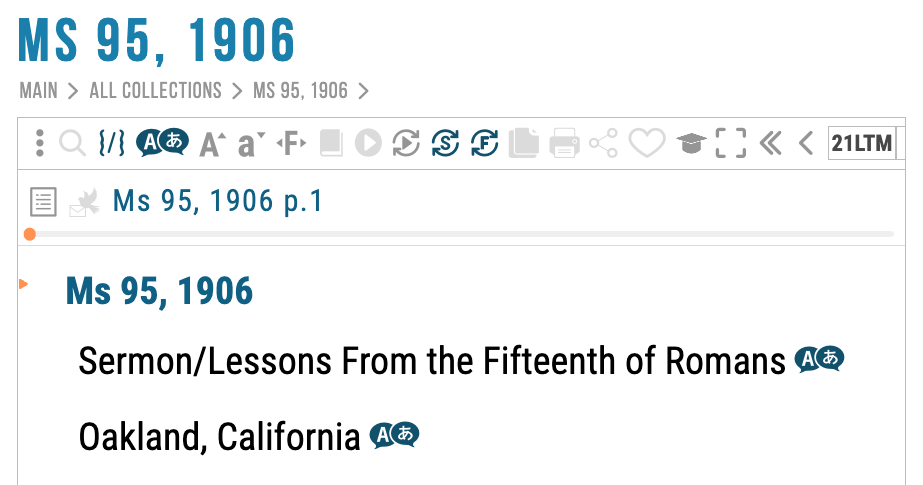
\includegraphics[width=1\linewidth]{images/sermons-and-talks.png}
    \label{fig:enter-label}
\end{figure}

Za nas, osobno, ovi citati su nepotvrđeni i, posebno, nevažeći u usporedbi s potvrđenim djelima Ellen White. Ali ako netko inzistira na jednako vrednovanju njenih nepotvrđenih izvještaja i objavljenih spisa, nećemo im stati na put, već ćemo dodatno potvrditi zaključak o Svetom Duhu kao biću. Slijedimo zajedno.

Čak i u usporedbi s potvrđenim spisima Ellen White, takav Sveti Duh, kao biće, ne bi bio jedno s Bogom jer je Krist bio \egwinline{\textbf{Jedino biće koje je bilo jedno s Bogom}}[Lt121-1897.7; 1897][https://egwwritings.org/read?panels=p7266.13]. Ovaj Sveti Duh, kao biće, ne bi mogao \egwinline{\textbf{ući u sve savjete i namjere Božje}}, zato jer je Krist bio \egwinline{\textbf{jedino biće}}[PP 34.1; 1890][https://egwwritings.org/read?panels=p84.75] koje je to moglo učiniti. Ovo Biće se ne treba uzdizati jer \egwinline{\textbf{Samo se Otac i Sin \underline{jedino} trebaju biti uzdignuti}}[YI, 7. srpnja 1898 par.2.; 1898][https://egwwritings.org/read?panels=p469.2964]. Sveti Duh, kao biće, ne bi se uklopio u poredak neba kao treće biće jer je Sotona bio \egwinline{\textbf{sljedeći do Krista najuzvišenije \underline{biće}} na nebeskim dvorovima}[RH 9. kolovoza 1898, par. 7; 1898][https://egwwritings.org/read?panels=p821.17145]. Ovaj Sveti Duh, kao biće, nije bio uključen u cijenu spasenja; niti je bio u savezu s Ocem i Sinom da spasi svijet, niti je bio obeščašćen čovjekovim prijestupom.

\egwinline{Veliki dar spasenja stavljen je u naš doseg uz \textbf{beskonačnu cijenu za Oca i Sina}.}[RH 21. studenog 1912, par. 2; 1912][https://egwwritings.org/read?panels=p821.33329]

\egwinline{U planu da se spasi izgubljeni svijet, savjet je bio između njih \textbf{\underline{obojice}}; \textbf{savez mira bio je između Oca i Sina}.}[ST 23. prosinca 1897, par. 2; 1897][https://egwwritings.org/read?panels=p820.14803]

\egwinline{Ali u prijestupništvu čovjeka \textbf{\underline{obojica} i Otac i Sin su bili obeščašćeni}.}[ST 12. prosinca 1895, par. 7; 1895][https://egwwritings.org/read?panels=p820.13243]

Takav Sveti Duh, kao biće, ne uklapa se u harmoniju s potvrđenim izvještajima Ellen White, niti s Svetim Pismom. Sveti Duh se naziva ‘\textit{duh}’, te je on eksplicitno duh.

Postoje nekoliko citata Sestre White koji potječu iz propovijedi ili govora koji su objavljeni nakon njezine smrti, a koriste se u dokazivanju da je sestra White naučavala i podupirala doktrinu o Trojstvu. U nastavku ćemo predstaviti nekoliko takvih. Pozivamo svakoga da odmjeri ove citate s njenim potvrđenim i objavljenim radom, onim tijekom njezina života.

“\textit{I tada se dodiruju zlatne harfe, i glazba teče kroz sve nebesko mnoštvo, i oni padaju ničice i štuju Oca i Sina i Svetoga Duha}.”\footnote{\href{https://egwwritings.org/?ref=en_Ms139-1906.32&para=9579.38}{EGW; Ms139-1906.32; 1906}} [Propovijed/Misli o Mateju 4. Oakland, Kalifornija 24. srpnja 1906.; Prethodno neobjavljeno.]

“\textit{Trebamo shvatiti da je Sveti Duh, koji je isto toliko osoba koliko je Bog osoba, hoda ovim prostorima.}”\footnote{\href{https://egwwritings.org/?ref=en_Ms66-1899.11&para=6622.19}{EGW; Ms66-1899.11: 1899}} [Govor/Izvaci iz govora koje je E. G. White održala na otvorenju College Hall, Avondale, i u crkvi Avondale]
